%!TEX root = main.tex

\section{Notes on category theoretic probability and string diagrams}

Category theoretic treatments of probability theory often start with \emph{probability monads} (for a good overview, see \citep{jacobs_probability_2018}). A monad on some category $C$ is a functor $T:C\to C$ along with natural transformations called the unit $\eta:1_C\to T$ and multiplication $\mu:T^2\to T$. Roughly, functors are maps between categories that preserve identity and composition structure and natural transformations are "maps" between functors that also preserve composition structure. The monad unit is similar to the identity element of a monoid in that application of the identity followed by multiplication yields the identity transformation. The multiplication transformation is also (roughly speaking) associative.

An example of a probability monad is the discrete probability monad given by the functor $\mathcal{D}:\textbf{Set}\to\textbf{Set}$ which maps a countable set $X$ to the set of functions from $X\to [0,1]$ that are probability measures on $X$, denoted $\mathcal{D}(X)$. $\mathcal{D}$ maps a measurable function $f$ to $\mathcal{D}f:X\to \mathcal{D}(X)$ given by $\mathcal{D}f:x\mapsto \delta_{f(x)}$. The unit of this monad is the map $\eta_X:X\to \mathcal{D}(X)$ given by $\eta_X:x\mapsto \delta_x$ (which is equivalent to $\mathcal{D} 1_X$) and multiplication is $\mu_X:\mathcal{D}^2(X)\to \mathcal{D}(X)$ where $\mu_X:\Omega\mapsto \sum_{\phi} \Omega(\phi) \phi$.

For continuous distributions we have the Giry monad on the category $\textbf{Meas}$ of mesurable spaces given by the functor $\mathcal{G}$ which maps a measurable space $X$ to the set of probability measures on $X$, denoted $\mathcal{G}(X)$. Other elements of the monad (unit, multiplication and map between morphisms) are the ``continuous'' version of the above.

Of particular interest is the Kleisli category of the monads above. The Kleisli $C_T$ category of a monad $T$ on category $C$ is the category with the same objects and the morphisms $X\to Y$ in $C_T$ is the set of morphisms $X\to TY$ in $C$. Thus the morphisms $X\to Y$ in the Kleisli category $\textbf{Set}_{\mathcal{D}}$ are morphisms $X\to \mathcal{D}(Y)$ in $\textbf{Set}$, i.e. stochastic matrices, and in the Kleisli category $\textbf{Meas}_{\mathcal{G}}$ we have Markov kernels. Composition of arrows in the Kleisli categories correspond to Matrix products and ``kernel products'' respectively.

Both $\mathcal{D}$ and $\mathcal{G}$ are known to be \emph{commutative} monads, and the Kleisli category of a commutative monad is a symmetric monoidal category.

Diagrams for symmetric monoidal categories consist of wires with arrows, boxes and a couple of special symbols. The identity object (which we identify with the set $\{*\}$) is drawn as nothing at all  $\{*\}:=\boxed{\hspace{2em}}$ and identity maps are drawn as bare wires:

\begin{align}
	\mathrm{Id}_X:=\begin{tikzpicture}[->]
	\path (0,0) node (A) {\hspace{1em}$X$}
	++(0,0.5) coordinate (B); 
	\draw (A.center) -- (B);
	\end{tikzpicture}
\end{align}

We draw Kleisli arrows from the unit (i.e. probability distributions) $\mu:\{*\}\to X$ as triangles and Kleisli arrows $\kappa:X\to Y$ (i.e. Markov kernels $X\to \Delta(\mathcal{Y})$) as boxes. We draw the Kleisli arrow $\mathds{1}_{X}:X\to\{*\}$ (which is unique for each $X$) as below
\begin{align}
	\mu:=
	\begin{tikzpicture}[->]
		\path (0,0) node[dist] (A) {$\mu$}
		++(0,0.5) node (B) {\hspace{2em}$X$};
		\draw (A)--(B.center);
	\end{tikzpicture}
	\hspace{2cm} \kappa:=
	\begin{tikzpicture}[->]
		\path (0,0) node[kernel] (A) {$\kappa$}
		++(0,0.5) node(B) {\hspace{2em}$Y$};
		\draw (A)--(B.center);
	\end{tikzpicture}
\end{align}

The product of objects in \textbf{Meas} is given by $(X,\mathcal{X})\cdot(Y,\mathcal{Y})=(X\times Y,\mathcal{X}\otimes\mathcal{Y})$, which we will often write as just $X\times Y$. Horizontal juxtaposition of wires indicates this product, and horizontal juxtaposition also indicates the tensor product of Kleisli arrows. Let $\kappa_1:X\to W$ and $\kappa_2:Y\to Z$:
\begin{align}
 (X\times Y,\mathcal{X}\otimes\mathcal{Y}) :=
 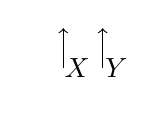
\begin{tikzpicture}[->]
	\path (0,0) node (A) {\hspace{1em}$X$}
	+(0,0.5) coordinate (B)
	++(0.5,0) node (C) {\hspace{1em}$Y$}
	+(0,0.5) coordinate (D); 
	\draw (A.center) -- (B);
	\draw (C.center) -- (D);
 \end{tikzpicture}
 \hspace{2cm} \kappa_1\otimes \kappa_2:=
 \begin{tikzpicture}
	\path (0,0) node (A) {\hspace{1em}$X$}
	+(0,0.5) node[kernel] (B) {$\kappa_1$}
	+(0,1) node (C) {\hspace{1em}$W$}
	++(0.8,0) node (D) {\hspace{1em}$Y$}
	+(0,0.5) node[kernel] (E) {$\kappa_2$}
	+(0,1) node (F) {\hspace{1em}$Z$}; 
	\draw (A.center) -- (B);
	\draw[->] (B) -- (C.center);
	\draw (D.center) --(E);
	\draw[->] (E) -- (F.center);
 \end{tikzpicture}
\end{align}

Composition of arrows is achieved by ``wiring'' boxes together. For $\kappa_1:X\to Y$ and $\kappa_2:Y\to Z$ we have


\begin{align}
\kappa_1\kappa_2(x;A)=\int_Y \kappa_2(y;A) \kappa_1(x;dy):=\begin{tikzpicture}
	\path (0,0) node (C) {\hspace{1em}$X$}
	++(0,0.5) node[kernel] (A) {$\kappa_1$}
	++(0,0.75) node[kernel] (B) {$\kappa_2$}
	++(0,0.5) node (D) {\hspace{1em}$Z$};
	\draw (C.center) -- (A);
	\draw (A) -- (B);
	\draw[->] (B) -- (D.center);
\end{tikzpicture}
\end{align}


Symmetric monoidal categoris have the following coherence theorem\citep{selinger_survey_2010}:

\begin{theorem}[Coherence (symmetric monoidal)]
	A well-formed equation between morphisms in the language of symmetric monoidal categories follows from the axioms of symmetric monoidal categories ifand only if it holds, up to isomorphism of diagrams, in the graphical language.
\end{theorem}

Isomorphism of diagrams for symmetric monoidal categories (somewhat informally) is any planar deformation of a diagram including deformations that cause wires to cross. We consider a diagram for a symmetric monoidal category to be well formed only if all wires point upwards.


In fact the Kleisli categories of the probability monads above have (for each object) unique \emph{copy}: $X\to X\times X$ and \emph{erase}: $X\to\{*\}$ maps that satisfy the \emph{commutative comonoid axioms} that (thanks to the coherence theorem above) can be stated graphically. These differ from the copy and erase maps of \emph{finite product} or \emph{cartesian} categories in that they do not necessarily respect composition of morphisms.


\begin{align}
	\text{Erase} = \mathds{1}_X := 
	\begin{tikzpicture}
	    \path (0,0) coordinate (A)
	    ++ (0,0.5) node(B) {};
	    \draw[-{Rays [n=8]}] (A) -- (B.center);
	\end{tikzpicture}
	\text{Copy} = x\mapsto \delta_{x,x} := 
	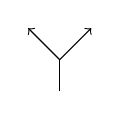
\begin{tikzpicture}[scale=0.8]
	\path (0,0) coordinate (A) 
	++ (0,0.5) coordinate (B)
	+ (0.5,0.5) coordinate (C)
	+ (-0.5,0.5) coordinate (D);
	\draw (A) -- (B);
	\draw[->] (B) -- (C);
	\draw[->] (B) -- (D);
	\end{tikzpicture}
\end{align}

\begin{align}
	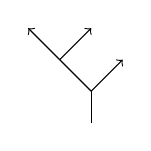
\begin{tikzpicture}[scale=0.8]
	\path (0,0) coordinate (A) 
	++ (0,0.5) coordinate (B)
	+ (0.5,0.5) coordinate (C)
	++ (-0.5,0.5) coordinate (D)
	+(0.5,0.5) coordinate (E)
	+(-0.5,0.5) coordinate (F);
	\draw (A) -- (B);
	\draw[->] (B) -- (C);
	\draw (B) -- (D);
	\draw[->] (D) -- (E);
	\draw[->] (D) -- (F);
	\end{tikzpicture}
	=
	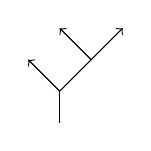
\begin{tikzpicture}[scale=0.8]
	\path (0,0) coordinate (A) 
	++ (0,0.5) coordinate (B)
	+ (-0.5,0.5) coordinate (C)
	++ (0.5,0.5) coordinate (D)
	+(0.5,0.5) coordinate (E)
	+(-0.5,0.5) coordinate (F);
	\draw (A) -- (B);
	\draw[->] (B) -- (C);
	\draw (B) -- (D);
	\draw[->] (D) -- (E);
	\draw[->] (D) -- (F);
	\end{tikzpicture}
	:=
		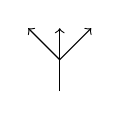
\begin{tikzpicture}[scale=0.8]
	\path (0,0) coordinate (A) 
	++ (0,0.5) coordinate (B)
	+ (-0.5,0.5) coordinate (C)
	+ (0,0.5) coordinate (D)
	+(0.5,0.5) coordinate (E);
	\draw (A) -- (B);
	\draw[->] (B) -- (C);
	\draw[->] (B) -- (D);
	\draw[->] (B) -- (E);
	\end{tikzpicture}\label{eq:ccom1}
\end{align}

\begin{align}
	\begin{tikzpicture}[scale=0.8]
	\path (0,0) coordinate (A) 
	++ (0,0.5) coordinate (B)
	+ (0.5,0.5) coordinate (C)
	+ (-0.5,0.5) node (D) {};
	\draw (A) -- (B);
	\draw[->] (B) -- (C);
	\draw[-{Rays [n=8]}] (B) -- (D);
	\end{tikzpicture}
	= 
	\begin{tikzpicture}[scale=0.8]
	\path (0,0) coordinate (A) 
	++ (0,0.5) coordinate (B)
	+ (0.5,0.5) node (C) {}
	+ (-0.5,0.5) coordinate (D) ;
	\draw (A) -- (B);
	\draw[-{Rays [n=8]}] (B) -- (C);
	\draw[->] (B) -- (D);
	\end{tikzpicture}
	=
	\begin{tikzpicture}[scale=0.8]
	\path (0,0) coordinate (A) 
	++ (0,1) coordinate (B);
	\draw[->] (A) -- (B);
	\end{tikzpicture}\label{eq:ccom2}
\end{align}

\begin{align}
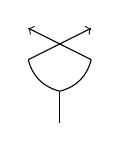
\begin{tikzpicture}[scale=0.8]
	\path (0,0) coordinate (A) 
	++ (0,0.5) coordinate (B)
	+ (0.5,0.5) coordinate (C)
	+ (-0.5,0.5) coordinate (D)
	+(0.5,1) coordinate (E)
	+(-0.5,1) coordinate (F);
	\draw (A) -- (B);
	\draw (B) to [bend right] (C);
	\draw (B) to [bend left] (D);
	\draw[->] (C) to  (F);
	\draw[->] (D) to  (E);	
\end{tikzpicture}
=
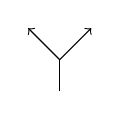
\begin{tikzpicture}[scale=0.8]
	\path (0,0) coordinate (A) 
	++ (0,0.5) coordinate (B)
	+ (0.5,0.5) coordinate (C)
	+ (-0.5,0.5) coordinate (D);
	\draw (A) -- (B);
	\draw[->] (B) -- (C);
	\draw[->] (B) -- (D);
\end{tikzpicture}\label{eq:ccom3}
\end{align}

Finally, $\{*\}$ is a terminal object in the Kleisli categories of either probability monad. This means that the map $X\to\{*\}$ is unique for all objects $X$, and as a consequence for all objects $X,Y$ and all $\kappa:X\to Y$ we have
\begin{align}
\begin{tikzpicture}
 \path (0,0) node (A) {\hspace{1em}$X$}
 ++(0,0.5) node[kernel] (B) {$\kappa$}
 ++(0,0.5) node (C) {};
 \draw (A.center) -- (B);
 \draw[-{Rays [n=8]}] (B) -- (C);
\end{tikzpicture}
=
\begin{tikzpicture}
 \path (0,0) node (A) {\hspace{1em}$X$}
  ++(0,0.5) node (C) {};
 \draw[-{Rays [n=8]}] (A.center) -- (C);
\end{tikzpicture}\label{eq:termobj}
\end{align}
This is equivalent to requiring for all $x\in X$ $\int_Y \kappa(x;dy)=1$. In the case of $\textbf{Set}_\mathcal{D}$, this condition is what differentiates a stochastic matrix from a general positive matrix (which live in a larger category than $\textbf{Set}_\mathcal{D}$).

Thus when manipulating diagrams representing Markov kernels in particular (and, importantly, not more general symmetric monoidal categories) diagram isomorphism also includes applications of \ref{eq:ccom1}, \ref{eq:ccom2}, \ref{eq:ccom3} and \ref{eq:termobj}.

A particular property of the copy map in $\textbf{Meas}_{\mathcal{G}}$ (and probably $\textbf{Set}_\mathcal{D}$ as well) is that it commutes with Markov kernels iff the markov kernels are deterministic \citep{fong_causal_2013}.

\subsection{Disintegration and Bayesian inversion}

\emph{Disintegration} is a key operation on probability distributions (equivalently arrows $\{*\}\to X$) in the categories under discussion. It corresponds to ``finding the conditional probability'' (though conditional probability is usually formalised in a slightly different way).

Given a distribution $\mu:\{*\}\to X\otimes Y$, a disintegration $c:X\to Y$ is a Markov kernel that satisfies
\begin{align}
	\begin{tikzpicture}
	 	\path (0,0) node[dist] (A) {$\mu$}
	 	+ (0,0.7) node (B) {$X$ $Y$};
	 	\draw ($(A.north) +(-0.2,0)$) -- ($(B.south) + (-0.2,0)$);
	 	\draw ($(A.north) +(0.2,0)$) -- ($(B.south) + (0.2,0)$);
	\end{tikzpicture}
	=
	\begin{tikzpicture}
	\path (0,0) node[dist] (A) {$\mu$}
	+ (0.2,0.5) node (Z) {}
	++ (-0.2,0.5) coordinate (B)
	+ (0.5,0.5) node[kernel] (C) {$c$}
	+ (-0.5,0.5) coordinate (D)
	+(0.5,1.2) node (E) {$Y$}
	+(-0.5,1.2) node (F) {$X$};
	\draw ($(A.north) +(-0.2,0)$) -- (B);
	\draw[-{Rays [n=8]}] ($(A.north) +(0.2,0)$) -- (Z);
	\draw (B) -- (C);
	\draw (B) -- (D);
	\draw (D) -- (F);
	\draw (C) -- (E);
	\end{tikzpicture}
\end{align}

Disintegrations always exist in $\textbf{Set}_{\mathcal{D}}$ but not in $\textbf{Meas}_{\mathcal{G}}$. The do exist in the latter if we restrict ourselves to standard measurable spaces. If $c_1$ and $c_2$ are disintegrations $X\to Y$ of $\mu$, they are equal $\mu$-A.S. In fact, this equality can be strengthened somewhat - they are equal almost surely with respect to any distribution that shares the ``$X$-marginal'' of $\mu$.


Given $\sigma:\{*\}\to X$ and a channel $c:X\to Y$, a Bayesian inversion of $(\sigma,c)$ is a channel $d:Y\to X$ such that
\begin{align}
	\begin{tikzpicture}
	\path (0,0) node[dist] (A) {$\sigma$}
	++ (0,0.5) coordinate (B)
	+ (0.5,0.5) node[kernel] (C) {$c$}
	+ (-0.5,0.5) coordinate (D)
	+(0.5,1.2) node (E) {$Y$}
	+(-0.5,1.2) node (F) {$X$};
	\draw (A) -- (B);
	\draw (B) -- (C);
	\draw (B) -- (D);
	\draw (D) -- (F);
	\draw (C) -- (E);
	\end{tikzpicture}
	=
	\begin{tikzpicture}
	\path (0,0) node[dist] (A) {$\sigma$}
	++ (0,0.5) node[kernel] (Z) {$c$}
	++ (0,0.5) coordinate (B)
	+ (-0.5,0.5) node[kernel] (C) {$d$}
	+ (0.5,0.5) coordinate (D)
	+(0.5,1.2) node (E) {$Y$}
	+(-0.5,1.2) node (F) {$X$};
	\draw (A) -- (Z);
	\draw (Z) -- (B);
	\draw (B) -- (C);
	\draw (B) -- (D);
	\draw (D) -- (E);
	\draw (C) -- (F);
	\end{tikzpicture}
\end{align}

We can obtain disintegrations from Bayesian inversions and vise-versa.

\citet{clerc_pointless_2017} offer an alternative view of Bayesian inversion which they claim doesn't depend on standard measurability conditions, but there is a step in their proof I didn't follow.

\subsection{Generalisations}

\citet{cho_disintegration_2019} make use of a larger ``CD'' category by dropping \ref{eq:termobj}. I'm not completely clear whether you end up with arrows being ``Markov kernels for general measures'' or something else (can we have negative arrows?). This allows for the introduction of ``observables'' or ``effects'' of the form 
\begin{tikzpicture}
 \path (0,0) coordinate (A)
 ++ (0,0.5) node[expectation] (B) {$f$};
 \draw (A) -- (B);
\end{tikzpicture}.

\citet{jacobs_causal_2019} make use of an embedding of $\textbf{Set}_\mathcal{D}$ in $\textbf{Mat}(\mathbb{R}^+)$ with morphisms all positive matrices (I'm not totally clear on the objects, or how they are self-dual - this doesn't seem to be exactly the same as the category of finite dimensional vector spaces). This latter category is compact closed, which - informally speaking - supports the same diagrams as symmetric monoidal categories with the addition of ``upside down'' wires.

\subsection{Key questions for Causal Theories}

We will first define \emph{labeled diagrams}. Rather than labelling the wires of our diagrams with \emph{spaces} (as is typical \citep{selinger_survey_2010}), we assign a unique label to each ``wire segment''. Somewhat informally, we assign a unique label to each bare wire in the diagram with the following additonal qualifications:
\begin{itemize}
	\item If we have a box in the diagram representing the identity map, the incoming and outgoing wires are given the same label
	\item If we have a wire crossing in the diagram, the diagonally opposite wires are given the same label
	\item The input wire and the \emph{two} output wires of the copy map are given the same label
\end{itemize}
Given two diagrams $G_1$ and $G_2$ that are isomorphic under transformations licenced by the axioms of symmetric monoidal categories and commutative comonoid axioms, suppose we have a labelling of $G_1$. We can label $G_2$ using the following translation rule:
\begin{itemize}
	\item For each box in $G_2$, we can identify a corresponding box in $G_1$ via labels on each box. For each such pair of boxes, we label the incoming wires of the $G_2$ box with the labels of the $G_1$ box preserving the left-right order. We do likewise for outgoing wires.
\end{itemize}

These rules will lead to a unique labelling of $G_2$ with all wire segments are labelled. We would like for these rules to yield the following:
\begin{itemize}
	\item For any sequence of diagram isomorphisms beginning with $G_1$ and ending with $G_2$, we end up with the same set of labels
	\item If we label $G_2$ according to the rules above then relabel $G_1$ from $G_2$ according to the same rules we retrieve the original labels of $G_1$
\end{itemize}

We do not prove these properties here, but motivate them via the following considerations:
\begin{itemize}
 	\item These properties obviously hold for the wire segments into and out of boxes
 	\item The only features a diagram may have apart from boxes and wires are wire crossings, copy maps and erase maps
 	\item The labeling rule for wire crossings respects the symmetry of the swap map
 	\item The labeling rule for copy maps respects the symmetry of the copy map and the property described in Equation \ref{eq:ccom3}
\end{itemize}

We will continue to follow the convention whereby ``internal'' wire labels are omitted from diagrams.

Note also that each wire that terminates in a free end can be associated with a random variable. Suppose for $N\in\mathbb{N}$ we have a kernel $\kappa:A\to \times_{i\in N} X_i$. Define by $\pi_j$ ($j\in[N]$) the projection map $\pi_j:\times_{i\in N}X_i\to X_j$ defined by $\pi_j:(x_0,...,x_N)\mapsto x_j$. $\pi_j$ is a measurable function, hence a random variable.

\paragraph{generalised disintegrations}: Of key importance to our work is generalising the notion of disintegration (and possibly Bayesian inversion) to general kernels $X\to Y$ rather than restricting ourselves to probability distributions $\{*\}\to Y$. We will define generalised disintegrations as a straightforward analogy regular disintegrations, but the conditions under which such disintegrations exist are more restrictive than for regular disintegraions.

A kernel $c:X\to Y$ is a \emph{generalised disintegration} (``g-disintegration'') of $\kappa$  from $X$ to $Y$ if the following holds:

\begin{align}
	\begin{tikzpicture}
	 	\path (0,0) coordinate (Z)
	 	++(0,0.5) node[kernel] (A) {\hspace{1em}$\kappa$}
	 	+ (0,0.7) node (B) {$X$ $Y$};
	 	\draw (Z) -- (A);
	 	\draw ($(A.north) +(-0.2,0)$) -- ($(B.south) + (-0.2,0)$);
	 	\draw ($(A.north) +(0.2,0)$) -- ($(B.south) + (0.2,0)$);
	\end{tikzpicture}
	=
	\begin{tikzpicture}
	\path (0,0) coordinate (X)
	++ (0,0.5) node[kernel] (A) {\hspace{1em}$\kappa$}
	+ (0.2,0.5) node (Z) {}
	++ (-0.2,0.5) coordinate (B)
	+ (0.5,0.5) node[kernel] (C) {$c$}
	+ (-0.5,0.5) coordinate (D)
	+(0.5,1.2) node (E) {$Y$}
	+(-0.5,1.2) node (F) {$X$};
	\draw (X) -- (A);
	\draw ($(A.north) +(-0.2,0)$) -- (B);
	\draw[-{Rays [n=8]}] ($(A.north) +(0.2,0)$) -- (Z);
	\draw (B) -- (C);
	\draw (B) -- (D);
	\draw (D) -- (F);
	\draw (C) -- (E);
	\end{tikzpicture}
\end{align}

In contrast to regular disintegrations, generalised disintegrations ``usually'' do not exist. Consider $D=X=Y=\{0,1\}$ and 
\begin{align}
	\kappa:\begin{cases} 1\mapsto \delta_1\otimes \delta_1\\
						 0\mapsto \delta_1\otimes \delta_0\end{cases}
\end{align}

There is clearly no kernel $c:X\to Y$ that simultaneously satisfies $\delta_1 c=\delta_1$ if $D=1$ and $\delta_0 c = \delta_0$ if $D=0$. Subject to some regularity conditions, we can define g-disintegrations of a canonically related kernel that do generally exist; intuitively, we g-disintegrations exist if they take the ``input wires'' of $\kappa$ as input wires themselves.

\begin{theorem}
For all $\kappa:D\to X\times Y$, if $D$ is countable and $X\times Y$ is standard measurable, a g-disintegration of $\kappa_{id}$ exists in the following three directions: from $D\to X\times Y$, from $D\times X\to Y$ and from $D\times Y\to X$. In general, a g-disintegration does not exist from $A\to B$ if 
\end{theorem}

\begin{proof}
For $D\to X\times Y$, we note that $\kappa$ is always a disintegration:

\begin{align}
\begin{tikzpicture}
 \path (0,0) node (A) {$D$}
 ++(0,0.35) coordinate (B)
 +(0,0.25) node[kernel] (C) {$\kappa$}
 +(0.5,0.25) coordinate (D)
 +(-0.15,0.8) node (X) {$X$}
 +(0.15,0.8) node (Y) {$Y$}
 +(0.5,0.8) node (Z) {$D$};
 \draw (A)--(B);
 \draw (B) -- (C);
 \draw (B) to [bend right] (D);
 \draw ($(C.north)+(-0.15,0)$) -- (X);
 \draw ($(C.north)+(0.15,0)$) -- (Y);
 \draw (D) -- (Z);
\end{tikzpicture}=
\begin{tikzpicture}
 \path (0,0) node (A) {$D$}
 ++(0,0.35) coordinate (B)
 +(0,0.25) node[kernel] (C) {$\kappa$}
 +(0.5,0.25) coordinate (D)
 +(-0.15,0.8) node (X) {}
 +(0.15,0.8) node (Y) {}
 ++(0.5,0.8) node[kernel] (Z) {$\kappa$}
 +(-0.15,0.8) node (X1) {$X$}
 +(0.15,0.8) node (Y1) {$Y$}
 +(0.5,0.8) node (D1) {$D$};
 \draw (A)--(B);
 \draw (B) -- (C);
 \draw (B) to [bend right] (D);
 \draw[-{Rays [n=8]}] ($(C.north)+(-0.15,0)$) -- (X);
 \draw[-{Rays [n=8]}] ($(C.north)+(0.15,0)$) -- (Y);
 \draw (D) -- (Z);
 \draw (D) to [bend right] (D1);
 \draw ($(Z.north)+(-0.15,0)$) -- (X1);
 \draw ($(Z.north)+(0.15,0)$) -- (Y1);
\end{tikzpicture}
\end{align}

Given $\kappa:D\to X\times Y$, define the \emph{canonical extension} $\kappa_{id}$:
\begin{align}
\kappa_{id} :=
\begin{tikzpicture}
 \path (0,0) node (A) {$D$}
 ++(0,0.35) coordinate (B)
 +(0,0.25) node[kernel] (C) {$\kappa$}
 +(0.5,0.25) coordinate (D)
 +(-0.15,0.8) node (X) {$X$}
 +(0.15,0.8) node (Y) {$Y$}
 +(0.5,0.8) node (Z) {$D$};
 \draw (A)--(B);
 \draw (B) -- (C);
 \draw (B) to [bend right] (D);
 \draw ($(C.north)+(-0.15,0)$) -- (X);
 \draw ($(C.north)+(0.15,0)$) -- (Y);
 \draw (D) -- (Z);
\end{tikzpicture}\label{eq:cextn}
\end{align}

The canonical extension takes a copy of the input and maps it to the output.

$D\times X\to Y$ and $D\times Y\to X$ are symmetric directions, so we will argue only for $D\times X\to Y$. For all $y\in D$ we have a disintegration $c_y:X\to Y$ of $\delta_y \kappa$ by standard measurability of $X\times Y$. Define $c:D\times X\to Y$ by $c:(y,x)\mapsto c_y(x)$. Clearly, $c(y,x)$ is a probability distribution on $Y$ for all $(y,x)\in D\times X$. It remains to show $c(\cdot)^{-1}(B)$ is measurable for all $B\in \mathcal{B}([0,1])$. But $c(\cdot)^{-1}(B) = \cap_{y\in D} c_y(\cdot)^{-1}(B)$. The right hand side is measurable by measurability of $c_y(\cdot)^{-1}(B)$ and the properties of a $\sigma$-algebra, so $c$ is a Markov kernel. By the definition of $c_y$, we have for all $y\in D$
\begin{align}
	\begin{tikzpicture}
	 	\path (0,0) node[dist] (Z) {$\delta_y$}
	 	++(0,0.3) coordinate (W)
	 	++(0,0.5) node[kernel] (A) {\hspace{1em}$\kappa$}
	 	+ (0,0.7) node (B) {$X$ $Y$}
	 	+ (0.6,0.7) node (C) {$D$};
	 	\draw (Z) -- (A);
	 	\draw ($(A.north) +(-0.2,0)$) -- ($(B.south) + (-0.2,0)$);
	 	\draw ($(A.north) +(0.2,0)$) -- ($(B.south) + (0.2,0)$);
	 	\draw (W) to [bend right] (C);
	\end{tikzpicture}
	&=
	\begin{tikzpicture}
	\path (0,0) node[dist] (X) {$\delta_y$}
	++ (0,0.3) coordinate (W)
	++ (0,0.5) node[kernel] (A) {\hspace{1em}$\kappa$}
	+ (0.2,0.5) node (Z) {}
	++ (-0.2,0.5) coordinate (B)
	+ (0.5,0.5) node[kernel] (C) {$c_y$}
	+ (-0.5,0.5) coordinate (D)
	+(0.5,1.2) node (E) {$Y$}
	+(-0.5,1.2) node (F) {$X$}
	+(1,1.2) node (G) {$D$};
	\draw (X) -- (A);
	\draw ($(A.north) +(-0.2,0)$) -- (B);
	\draw[-{Rays [n=8]}] ($(A.north) +(0.2,0)$) -- (Z);
	\draw (B) -- (C);
	\draw (B) -- (D);
	\draw (D) -- (F);
	\draw (C) -- (E);
	\draw (W) to [bend right] (G);
	\end{tikzpicture}\\
	&= 
	\begin{tikzpicture}
	\path (0,0) node[dist] (X) {$\delta_y$}
	++ (0,0.3) coordinate (W)
	++ (0,0.5) node[kernel] (A) {\hspace{1em}$\kappa$}
	+ (0.2,0.5) node (Z) {}
	++ (-0.2,0.5) coordinate (B)
	+ (0.5,0.5) node[kernel] (C) {$c$}
	+ (-0.5,0.5) coordinate (D)
	+(0.5,1.2) node (E) {$Y$}
	+(-0.5,1.2) node (F) {$X$}
	+(1,0) coordinate (G) 
	+(1,1.2) node (H) {$D$};
	\draw (X) -- (A);
	\draw ($(A.north) +(-0.2,0)$) -- (B);
	\draw[-{Rays [n=8]}] ($(A.north) +(0.2,0)$) -- (Z);
	\draw (B) -- (C);
	\draw (B) -- (D);
	\draw (D) -- (F);
	\draw (C) -- (E);
	\draw (W) to [bend right] (G);
	\draw (G) -- (H);
	\draw (G) to [bend left] (C);
	\end{tikzpicture}
\end{align}
Which implies
\begin{align}
\begin{tikzpicture}
 	\path (0,0) node (Z) {}
 	++(0,0.3) coordinate (W)
 	++(0,0.5) node[kernel] (A) {\hspace{1em}$\kappa$}
 	+ (0,0.7) node (B) {$X$ $Y$}
 	+ (0.6,0.7) node (C) {$D$};
 	\draw (Z) -- (A);
 	\draw ($(A.north) +(-0.2,0)$) -- ($(B.south) + (-0.2,0)$);
 	\draw ($(A.north) +(0.2,0)$) -- ($(B.south) + (0.2,0)$);
 	\draw (W) to [bend right] (C);
	\end{tikzpicture}
	&=
	\begin{tikzpicture}
	\path (0,0) node (X) {}
	++ (0,0.3) coordinate (W)
	++ (0,0.5) node[kernel] (A) {\hspace{1em}$\kappa$}
	+ (0.2,0.5) node (Z) {}
	++ (-0.2,0.5) coordinate (B)
	+ (0.5,0.5) node[kernel] (C) {$c$}
	+ (-0.5,0.5) coordinate (D)
	+(0.5,1.2) node (E) {$Y$}
	+(-0.5,1.2) node (F) {$X$}
	+(1,0) coordinate (G) 
	+(1,1.2) node (H) {$D$};
	\draw (X) -- (A);
	\draw ($(A.north) +(-0.2,0)$) -- (B);
	\draw[-{Rays [n=8]}] ($(A.north) +(0.2,0)$) -- (Z);
	\draw (B) -- (C);
	\draw (B) -- (D);
	\draw (D) -- (F);
	\draw (C) -- (E);
	\draw (W) to [bend right] (G);
	\draw (G) -- (H);
	\draw (G) to [bend left] (C);
	\end{tikzpicture}
\end{align}
 
Note that the only other (non-trivial) disintegrations do not feature $D$ as an ``input wire''. All such 

\end{proof}

\paragraph{Conjecture:} This can be generalised to any $\kappa$ that is determined by its values on a countable set of points along with some notion of continuity. This seems likely to be true. In a more general setting, I think I could find a counterexample, but the converse also seems unlikely.

The extension of \emph{conditional independence} to g-disintegrations becomes a directional relationship. Suppose we have $\kappa:D\to X\times Y$ and a disintegration $c:D\times X\to Y$. We say $Y$ is directionally conditionally independent (DCI) of $D$ given $X$ if

Generalised disintegrations facilitate the following construction of a ``graphical model'':

Suppose we have two causal theories, $\mathscr{T}^*$ and $\mathscr{T}$ both with signature $E\times D\rightarrowtriangle E$, and $\mathscr{T}$ is a decision randomised version of $\mathscr{T}^*$ (i.e. $\mathscr{T}=\{(\lambda\kappa,\mu)|(\kappa,\mu)\in\mathscr{T}^*\}$ for some $\lambda:D\to D$. We will construct a graphical model from $\mathscr{T}^*$ and $\mathscr{T}$ in three steps:

First, we assume \emph{reproducibility} in the stronger theory $\mathscr{T}^*$. That is, for all $(\kappa,\mu)\in \mathscr{T}^*$ we suppose there exists $\gamma\in \Delta(\mathcal{D})$ such that $\gamma\kappa=\mu$. 

\todo{I don't think reproducibility is quite the right assumption, but it is good enough for now}

Second, we will assume certain \emph{generalised conditional independences} hold for the stronger theory $\mathscr{T}^*$ (we have not defined these, but they are the obvious generalisation of standard conditional independence lifted to g-disintegrations). Because we're constructing a graphical model, we will assume these are a ``DAG-compatible'' set, though we are under no obligation to do so. I conjecture we can illustrate these independences graphically. Suppose we have random variables $\RV{X}:E\to X$, $\RV{Y}:E\to Y$ and $\RV{Z}:E\to Z$, and we assume we have at least the generalised CIs implied by the following diagram for all $(\kappa,\mu)\in \mathscr{T}^*$:
\begin{align}
\kappa=\begin{tikzpicture}
\path (0,0) node (A) {$E$}
	++(0,0.2) coordinate (B)
	++ (0,0.3) node[kernel] (C) {\hspace{1em}$\kappa$}
	+ (0,0.5) node (D) {}
	+ (0.2,0.5) node (E) {}
	++ (-0.2,0.5) coordinate (F)
	+ (-0.5,0.5) node (G) {$X$}
	++ (0.5,0.5) node[kernel] (H) {$c_{Y|X}$}
	+ (-0.5,0.8) node (I) {$Y$}
	++(0.5,0.8) node[kernel] (J) {$c_{Z|Y}$}
	++(0,0.8) node (K) {$Z$};
	\draw (A) -- (B);
	\draw (B) -- (C);
	\draw[-{Rays [n=8]}] (C) -- (D);
	\draw[-{Rays [n=8]}] (C) -- (E);
	\draw (C) -- (F);
	\draw (F) -- (G);
	\draw (F) -- (H);
	\draw (H) -- (I);
	\draw (H) -- (J);
	\draw (J) -- (K);
\end{tikzpicture}
\end{align}


The above diagram is typed incorrectly, but we can always construct a kernel $\kappa_{\RV{XYZ}}$ that maps to $X\times Y\times Z$.